\documentclass[../MA_Thesis.tex]{subfiles}
\renewcommand{\baselinestretch}{1.5} 
\usepackage{hyperref}
\usepackage{csquotes}

\begin{document}

\subsection*{The Psychology of Moods}
Psychologists often consider state-level mood experiences to be multidimensional. Notably, \textcite{yik_structure_1999} successfully integrated four two-dimensional mood models (each based on the bipolar dimensions of \textit{pleasant-unpleasant} and \textit{activated-deactivated}) into a unified framework, demonstrating substantial overlap among these models when controlling for measurement errors. This two-dimensional model, visually illustrated by \textcite{feldman_variations_1995}'s circumplex model of mood adapted from \textcite{russell_circumplex_1980}'s model\footnote{Note: here \textit{arousal} can be considered as a similar construct as \textit{activation}.} (see Figure \ref{fig: mood circumplex}), has since been widely adopted in empirical research to explore the unique and joint effects of valence and activation. For example, \textcite{balch_dimensions_1999} examined how these mood dimensions influence word recall under different mood conditions, and \textcite{nealis_positive_2016} studied the role of affective valence and activation in replenishing self-control resources within an ego-depletion framework. Further challenging the traditional view of activation and valence as independent, the concept of \textit{core affect} integrates these dimensions, underscoring how activation levels can influence perceived pleasantness or unpleasantness of stimuli (\cite{petrolini_core_2020}; \cite{russell_core_1999}).

\begin{figure}
    \centering
    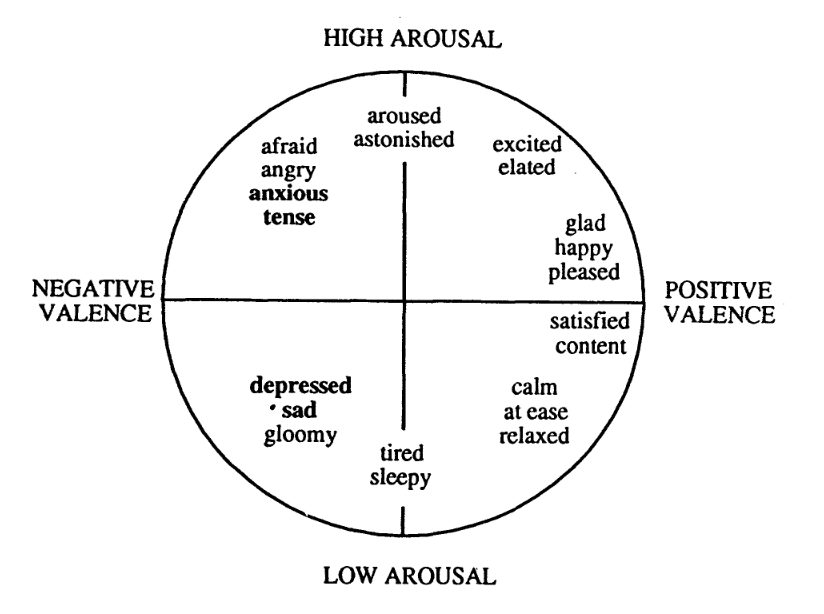
\includegraphics[width=0.5\linewidth, keepaspectratio]{screenshots/A Circumplex Model of Mood.png}
    \caption{Valence/Arousal Circumplex Model of Mood (\cite{feldman_variations_1995})}
    \label{fig: mood circumplex}
\end{figure}

A unified mood classification framework has advanced the understanding of the cognitive and behavioral consequences of mood states (\cite{lischetzke_mood_2022}). For instance, research on mood congruency illustrates how pleasant moods tend to bias actions towards positive content, while unpleasant moods do the opposite, influencing mood regulation strategies as described in \textcite{larsen_toward_2000}'s control theory model. Furthermore, mood affects both the content and the process of cognition (\cite{forgas_chapter_2017}). Positive moods improve the recall of positive information and broaden attention spans, facilitating creative and broad-concept learning. In contrast, negative moods promote detailed-oriented thinking, enhancing recall of negative information and learning that requires meticulous attention. Positive moods also lead to more generous social judgments, affecting interpersonal evaluations and interactions (\cite{forgas_mood_1995}). This body of research illustrates how mood influences cognitive processes, including memory, attention, learning, and social judgments, emphasizing the dynamic interplay between mood and cognitive function.

\subsection*{Demystifying creativity} 
Psychological and cognitive theories on creativity have shifted from mystical views of creativity to scientific explorations based on observable and measurable cognitive functions (\cite{finke_creative_1996}). An important milestone is the growing appreciation that, while creativity is often seen as a trait belonging only to exceptionally gifted individuals, it actually forms a fundamental aspect of human cognitive abilities, demonstrated by our versatile application of language, ability to form and apply new mental categories to organize our experiences, and skill in mentally handling objects (\cite{ward_creative_1999}). This evolution is supported by theoretical and empirical advancements that elucidate specific cognitive processes that lead to creative insights (\cite{finke_creative_1996}).

Amid this background, the field has witnessed the evolution of theoretical accounts to illuminate the cognitive systems that underlie creative thinking (\cite{johnson_divergent_2022}). One enduring theory is \textcite{mednick_associative_1962}'s associative theory, which suggests that creativity stems from the ability to form associations between disparate concepts in memory, where more creative individuals form equally strong connections between common and uncommon concepts, enabling novel associations. Advancements in cognitive neuroscience have further refined this view, with \textcite{dietrich_cognitive_2004} emphasizing that creativity relies on cognitive abilities such as attention, working memory, and cognitive flexibility, pinpointing specific brain circuits that underlie various creative processes. These insights have helped distinguish between deliberate and spontaneous modes of creativity, showing how these modes affect neural activity related to cognitive and emotional functions.

Building on these insights, the Creative Cognition Approach (\cite{kaufman_cambridge_2010}) details how basic cognitive operations---attention, perception, memory, reasoning---are utilized to generate innovative ideas. This framework extends \textcite{dietrich_cognitive_2004}'s findings by emphasizing the role of an individual’s knowledge depth and breadth in enhancing creative potential. It advocates for specific cognitive mechanisms such as analogical thinking and problem-solving that leverage this knowledge to foster creative outcomes.

Over the years, various theories have highlighted the stage-like nature of creative processes, commonly dividing them into two primary phases: 1) generating ideas and assessing their usefulness and 2) modifying them to meet specific creative goals (\cite{johnson_divergent_2022}). A notable example is the Geneplore model (\cite{finke_creative_1996}). This model posits that creative tasks begin with the generation of preliminary ideas, termed "preinventive" because they are not yet fully developed but possess potential for originality and applicability. The process involves alternating between generating and exploring these ideas, continuously refining them to conform to the specific requirements or constraints of the task (\cite{patterson_personal_2004}).

\textcite{nijstad_dual_2010}'s dual pathway to creativity model is another influential theory that focuses on the creative ideation process. It conceptualizes creativity as a constrained stochastic process characterized by random variation and selective retention (\cite{simonton_creativity_2000}). This model integrates aspects of the Geneplore model, which views creativity as a cognitive process that involves problem solving and memory retrieval, and also recognizes the importance of remote associations in creative thinking (\cite{mednick_associative_1962}). Specifically, it identifies two primary pathways: \textit{cognitive flexibility} and \textit{cognitive persistence}. Cognitive flexibility, often enhanced by positive mood states, allows easy switching between thoughts, aiding the exploration and connection of diverse ideas. This pathway is supported by neurophysiological features, such as the presence of dopamine in certain brain areas and reduced levels of latent inhibition, which allow more distant associations to enter working memory, thereby fostering originality. In contrast, cognitive persistence focuses on a deep, systematic exploration of fewer ideas, enhanced by negative moods that promote detailed attention and perseverance. This process involves the prefrontal cortex, particularly the dorsolateral areas involved in executive functions such as working memory and sustained attention.

\subsection*{Mood-Creativity Linkage}
It shall be no surprise that research on the cognitive consequences of mood has intersected with studies on creativity. Extensive psychological research has examined how different mood states influence creativity. \textcite{de_dreu_hedonic_2008} note that mood is one of the most studied and reliable predictors of creativity. While many studies suggest that positive moods elicit more creative responses than neutral moods, the comparison between positive and negative moods is less conclusive (\cite{de_dreu_hedonic_2008}). Some research indicates that positive moods enhance creativity more than negative moods (\cite{grawitch_effects_2003}), while others find similar levels of creativity in moods (\cite{bartolic_effects_1999}), or even greater creativity in negative moods (\cite{madjar_preliminary_2002}).

Given the bipartite dimensions of mood states (i.e., valence and activation; \cite{yik_structure_1999}), these inconsistencies may arise from a focus primarily on valence. Different cognitive processes leading to creativity (\cite{finke_creative_1996}; \cite{nijstad_dual_2010}) may also explain these contradictory results. In this sense, the dual pathway to creativity model (\cite{de_dreu_hedonic_2008}) distinguishes itself among the various theoretical frameworks that reconcile the inconsistent findings by recognizing the dimensions of valence and activation of mood and proposing \textit{flexibility} and \textit{persistence} pathways as distinct yet interrelated cognitive processes behind creative thinking. Specifically, this model posits that positive hedonic tones increase openness and receptiveness, enhancing cognitive flexibility, while negative tones narrow focus, boosting cognitive persistence. Activating moods, regardless of hedonic tone, generally lead to higher levels of creativity compared to deactivating moods due to increased mental and physical energy.

Moreover, the dual pathway to creativity model delineates how mood states enhance or hinder creative output in various ideation tasks (e.g., divergent thinking tasks) by integrating broader psychological theories. It highlights that creative fluency and originality emerge from enhanced cognitive flexibility, increased persistence, or a combination of both (\cite{nijstad_dual_2010}). Research from stress performance studies, psychophysiology, and neuroimaging suggests that activating moods significantly bolster creative fluency and originality compared to deactivating moods (\cite{de_dreu_hedonic_2008}). Furthermore, integrating the cognitive tuning model (\cite{schwarz_happy_1991}), the broaden-and-build theory (\cite{fredrickson_role_2001}), and the insights from studies on visual and conceptual focusing (\cite{derryberry_hemispheric_1989}), the dual pathway to creativity model argues that activating moods with a positive tone primarily enhance creativity through increased cognitive flexibility, whereas activating moods with a negative tone foster creativity through heightened persistence. Finally, although no significant differences are expected between positive activating moods (e.g., happiness) and negative activating moods (e.g., anger) in terms of fluency and originality, positive activating moods contribute to broader and more diverse cognitive categories, facilitating faster completion times in creative tasks. Negative activating moods tend to generate more ideas within specific cognitive categories, leading to longer completion times (\cite{de_dreu_hedonic_2008}).


\subsection*{Experimental Mood Induction}
One necessary condition to empirically test the link between mood and creativity is to effectively induce mood changes, allowing researchers to unravel the \textit{unique} effects of mood states on creativity. Experimental mood induction has been shown to be effective in altering mood (\cite{westermann_relative_1996}) and thus offers stronger evidence of the causal effects of mood states on creativity. Providing a more controlled and quantifiable approach, experimental mood induction surpasses self-reported questionnaires, which suffer from 1) inherent biases such as response styles and memory recall issues and 2) fundamentally correlational nature that often complicate accurate assessment (\cite{soubelet_influence_2011}).

There are a myriad of experimental mood induction methods, including imagination, films, sound and music, images, reading and writing passages, embodiment, virtual reality, feedback on performance tasks, self-referent statements, social interaction, physiological manipulations, and motivated performance tasks (\cite{lischetzke_mood_2022, maryam_fakhrhosseini_affectemotion_2017}). \textcite{siedlecka_experimental_2019} provides a classification framework for these techniques, categorizing them into visual stimuli, music, autobiographical recall, situational procedures, and imagery, which is crucial to understanding the effectiveness of various mood induction methods, helping researchers select the appropriate methodologies to investigate the impact of mood on behavior. \textcite{siedlecka_experimental_2019} found that images or videos are particularly effective in evoking a wide range of emotions, while music strongly elicits happiness, fear, and sadness. Autobiographical recall effectively induces anger, happiness, fear, disgust, and sadness. Creating social or physical situations elicits anger, surprise, fear, and happiness, and guided mental visualization is effective in inducing anger, happiness, disgust, sadness, and fear.

In addition to evaluating the effectiveness of various mood induction techniques, there has also been significant discussion on additional considerations for implementing mood induction experiments. For instance, implementing mood induction experiments requires precision in instructions and the choice of induction method to ensure the target mood state is effectively induced (\cite{maryam_fakhrhosseini_affectemotion_2017, siedlecka_experimental_2019}). Moreover, combining self-report and physiological measures can capture a more accurate picture of mood state (\cite{quigley_inducing_2014, siedlecka_experimental_2019}). Ethical considerations are also crucial, especially when inducing negative mood states. It is essential to ensure voluntary participation and comprehensive debriefing (\cite{maryam_fakhrhosseini_affectemotion_2017, quigley_inducing_2014, siedlecka_experimental_2019}).

\subsection*{Common Methods to Measure Creativity}
Apart from mood induction, another necessary condition to empirically test the mood-creativity linkage is choosing appropriate methods to measure creativity. Given the multifaceted nature of creativity (\cite{de_alencar_theory_2021}), researchers have developed diverse methodologies, including psychometric tests, observational methods, self-assessment techniques, and dynamic approaches to measure creativity in real-time or natural settings (\cite{kaufman_cambridge_2010}). However, defining what should be measured remains challenging due to creativity's complexity involving cognitive processes, personality traits, and environmental influences.

Fortunately, creativity scholars have proposed framework/taxonomy of creativity measurement that helps identify the most appropriate creativity measures for researchers' specific needs. For example, \textcite{batey_measurement_2012} proposed a heuristic framework for measuring creativity at multiple levels, guiding researchers in selecting the appropriate methods. This framework includes three dimensions: levels of creativity assessment (individual, team, organizational, cultural), facets of creativity assessment (trait, process, press, product), and measurement approaches (objective, self-rated, other-rated). Furthermore, \textcite{weiss_improved_2021} proposed a taxonomy of creativity assessment tools, detailing attributes including the measurement approach (self-report, other-report, ability tests), construct type (e.g., creative interests, achievements, divergent thinking), the type of generated data, scoring methods, and psychometric issues.

Despite the challenges in capturing the multifaceted nature of creativity, the field of creativity has seen extensive development, including refined traditional tests, technology-based assessments, and ecologically valid measures (\cite{kaufman_cambridge_2010}). Methodological approaches grounded in disciplines such as network science have been used to model semantic memory and test the associative theory of creativity. For instance, studies by \textcite{kenett_investigating_2014} and \textcite{beaty_forward_2021} show that greater semantic distance from a conventional idea increases the likelihood of a new idea being considered creative. \textcite{kenett_flexibility_2018} discuss the resilience of semantic memory networks, indicating greater flexibility in highly creative individuals. In addition, advances in computational linguistics and deep learning also contribute to creativity research. For example, \textcite{zedelius_beyond_2019} use linguistic properties, rather than subjective scoring, to measure creativity in writing. \textcite{johnson_divergent_2022} employ BERT-embedded representations to gauge narrative connections and \textcite{patterson_multilingual_2023} develop automatic scoring systems for divergent thinking tasks across multiple languages.

It is also worth mentioning that the field of creativity research stands on the cusp of several promising developments. As highlighted by \textcite{kaufman_cambridge_2010}, future creativity research should focus on innovative assessment methodologies that capture the dynamic nature of creative processes, such as real-time data collection techniques to digitally track creative activities and artificial intelligence techqniues to analyze patterns in creative output. Furthermore, cross-disciplinary approaches that integrate psychology, sociology, educational science, and neuroscience are essential to develop holistic and applicable measures across different cultural contexts, enriching our understanding of creativity and its manifestations.
\end{document}